\documentclass[10pt,twocolumn]{article} 
\usepackage{graphicx}
\usepackage{amssymb}
\usepackage{url,hyperref}

\begin{document}

\section{Implementation}

Moving from simulation to implementation on physical devices can reveal unforeseen challenges to the design, protocols, or experimental conditions around which a system is developed. We therefore see the real implementation, in addition to the simulation, as a necessary step to demonstrating our system's usefulness and effectiveness; for that reason we have implemented our system both on the NS3 simulation platform and on real Android mobile devices.

The Android platform represented 80\% of the mobile device market in 2014 and is expected to maintain three quarters of the global market share during the following four years cite International Data Corporation http://www.idc.com/getdoc.jsp?containerId=prUS24857114. We feel that targeting Android gives the most realistic view of what capabilities are available, now or in the future, for novel mobile systems.

The core system functionality is implemented as a standalone C++ module that can be built as an external library or into an application. The core library contains all of the platform-agnostic functionality and accesses platform resources via abstract interfaces.

Cross-platform support is fundamental to our software design: we can support NS3, Android, POSIX, and WinNT with no modifications to the core module. A thin platform-specific wrapper provides access to the environment, as seen in Figure \ref{fig:android-platform-wrapper}.

\begin{figure}[!b]
  \begin{center}
    \includegraphics[width=0.45\textwidth]{android-platform-wrapper.pdf}
  \end{center}

  \caption{\small The implementation architecture abstracts platform resources away from the core functionality for platform independence.}
  \label{fig:android-platform-wrapper}
\end{figure}

NS3 and Android differ in important ways; for one, the NS3 simulator uses only a single thread of execution for numerous application instances while Android offers many threads of execution for a single application instance. To be maximally flexible to different test environments or deployments, the core system logic is implemented in terms of the following abstractions:

\paragraph{Clock} gives access to the current time and date. In NS3 this reflects the simulation time, but in all other implementations it reflects the system clock.

\paragraph{Async} provides a mechanism for the core module to create tasks that may be run in the background, in the future, or periodically. Task scheduling and parallelism, if any, is defined by the implementation. The core functionality is thus scalable across many threads of execution as it operates in terms of decoupled tasks.

\paragraph{Cache} is how the core module stores and loads data, in lieu of files or databases. Caches of varying persistence are provided that may be implemented in volatile memory, on a hard disk, or in flash memory on a mobile device. The caching policies may vary given the storage medium and expected persistence of cached data.

\paragraph{Links} represent logical network connections and are abstracted as message queues. The implementation defines the network device and access mode of a particular link. The link layer aggregates one or more links into the logical network view held by the core logic.

\end{document}
